\section{Results and Conclusions}
\label{sec:make}

\subsection{data}
  \label{sec:America}
  The data collected for the star's magnitude is graphically displayed in the following depiction.
  \begin{figure}[H]
    \centering
    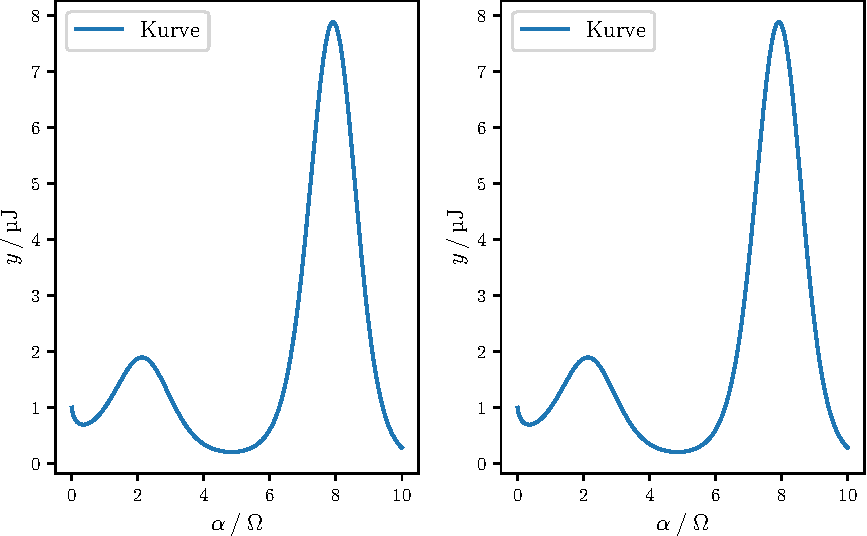
\includegraphics{plot.pdf}
    \caption{Magnitude of SW Lacertae}
  \end{figure}
  Additionally, data from the two comparison stars was taken and 
  the uncertainties are calculated with the package uncertainties from python.

\subsection{Ensemble Photometry}
  \label{sec:great}
  In order to excluded errors caused from different exposures of light, caused by traffic 
  or other unforseeable factors, the method of comparison stars is used. 
  Hence, not the magnitude of the star is evaluated, but the difference between the 
  star’s and the magnitude of the comparison stars. For this study of 
  SW Lacertae, the stars (1) TYC 3215-1586-1 and (2) TYC 3215-1406-1 were chosen as comparison stars. 
  In the following image, their position in the sky in relation to SW Lacertae
  is shown.
  \begin{figure}[H]
    \centering
    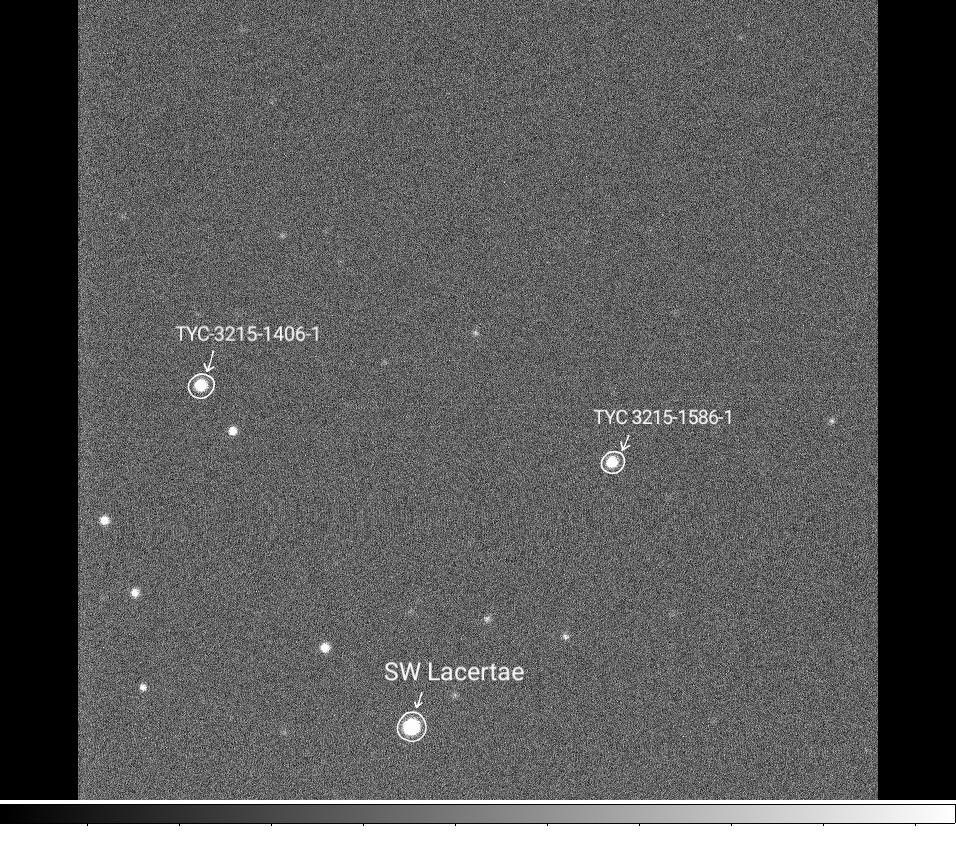
\includegraphics[width=200pt]{WestHA~2.jpg}
    \hspace{1em}
    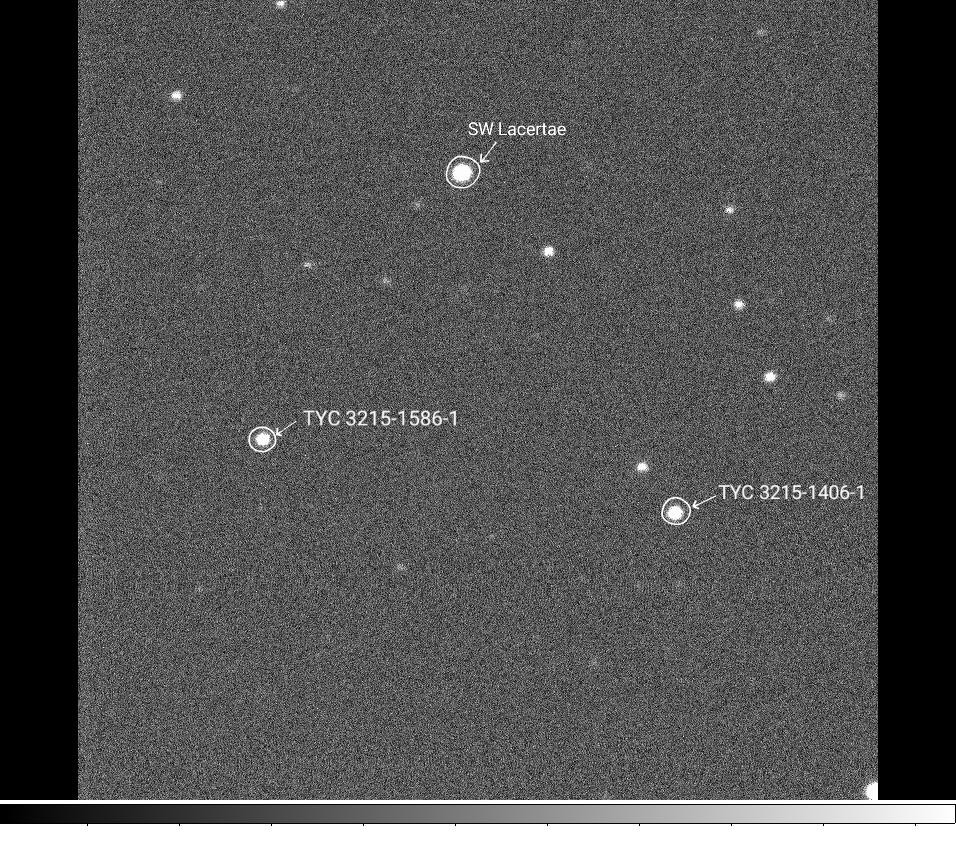
\includegraphics[width=200pt]{EastHA~2.jpg}
    \caption{Position of comparison stars in the sky; western sky on the left, eastern sky on the right}
    \label{fig:plot}
  \end{figure}
  The comparison to two stars was mainly used to reduce the likelihood of 
  variation in the comparison star brightness and other intruding factors.
  This has to be done for each filter seperately, because of the different 
  exposure times and the different colors of the stars.
  The resulting data for the V-filter is shown in the following plot.
  \begin{figure}[H]
    \centering
    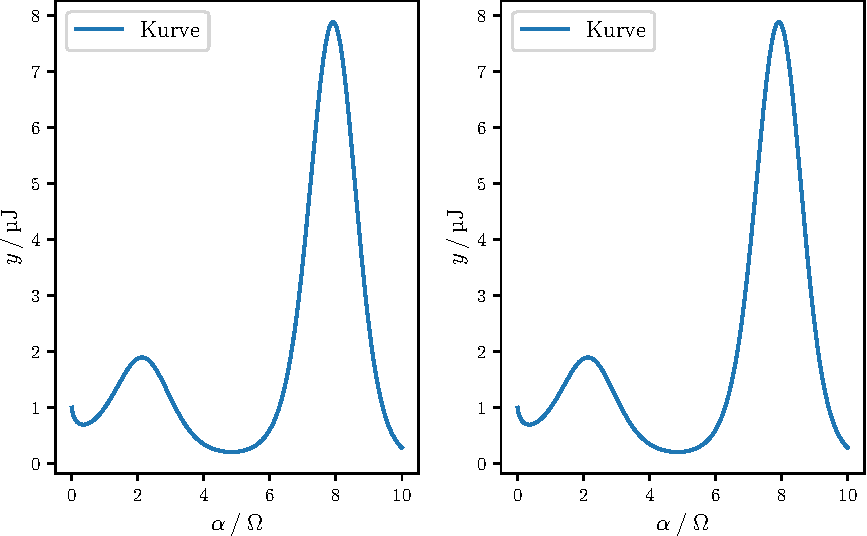
\includegraphics{plot.pdf}
    \caption{Magnitude Difference between SW Lacertae and TYC 3215-1586-1}
    \label{fig:plot}
  \end{figure}

\subsection{Phase}
  \label{sec:again}
  In order to obtain the phase in relation to an earlier measured phase, the epoch 
  \begin{equation*}
    E_{measurements} = HJD - 240000000
  \end{equation*}
  is calculated in a first step. The data for an earlier Minimum were provided by the 
  instructions for this lab. 
  \begin{align*}
    E_{min} = 49594.4684\\
    period = 0.3207209
  \end{align*}
  The phase in comparison to the given data is retrieved through the formula
  \begin{equation}
    phase = \dfrac{((E_{measurements}-E_{min})\ \% \ period)}{period}.
  \end{equation}
  This leads us to the following results:
  \begin{figure}[H]
    \centering
    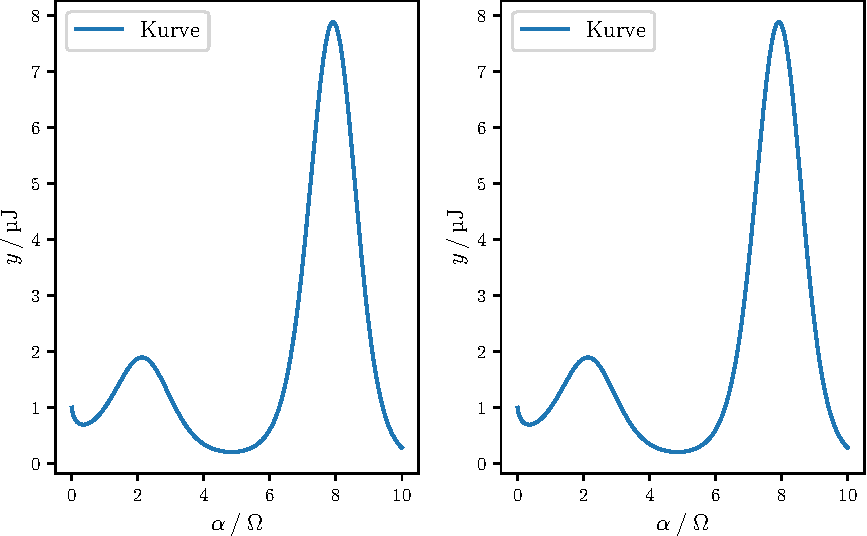
\includegraphics{plot.pdf}
    \caption{Magnitude against the Phase}
    \label{fig:phase}
  \end{figure}
  In this graphic, data gathered from another goup is included. %%%%%%%%%%%%%%%%%%%%%%%%%%%%%%%%%%%%%%%find out names
  They observed this binary star system at the same observatory at the %%%%%%%%%%%%%%%%%%%%%%%%%find out date

\subsection{Conclusion}
  \label{sec:fuckoff}
  On account of difficulties, which occured while recording the data, a full period could not
  be observed. The conclusions base therefore mostly on the data, collected by the other team.
  Saying this, the data of both observation nights fits perfectly to each other and therefore, 
  it can be presumed, that the others group data will deliver results, which match those of our 
  observations.\\
  It can be clearly seen in plot \ref{fig:phase}, that there is an offset of the first minimum 
  and $phase = 0$. That implies a period change of the system. This developement should be 
  further researched, because it could lead to new knowlegde on mass transfer of contact binary
  star systems.

\subsection{Discussion}
  \label{sec:orange}




Siehe \autoref{fig:plot}!
